\documentclass[border=8pt]{standalone}
\usepackage[T1]{fontenc}
\usepackage[utf8]{inputenc}
\usepackage{pgfplots}
\pgfplotsset{compat=1.18}
\usepackage{xcolor}

\definecolor{autcol}{HTML}{4C72B0}
\definecolor{abicol}{HTML}{55A868}
\definecolor{fxlcol}{HTML}{DD8452}

\begin{document}
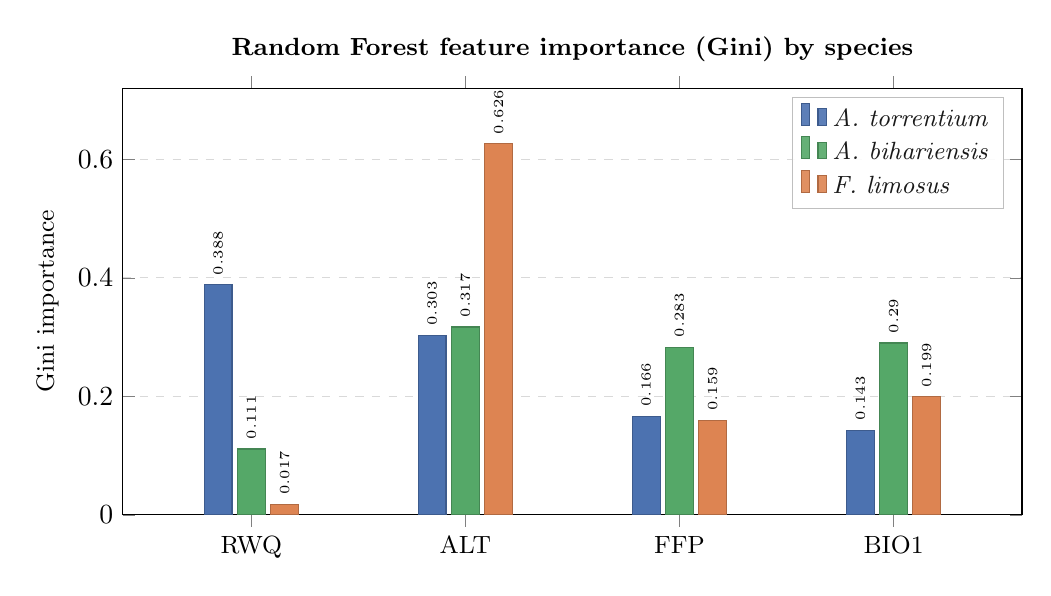
\begin{tikzpicture}
\begin{axis}[
  width=13cm, height=7cm,
  title={Random Forest feature importance (Gini) by species},
  title style={font=\bfseries\small},
  ybar,
  bar width=10pt,
  ylabel={Gini importance},
  ylabel style={font=\small},
  symbolic x coords={RWQ, ALT, FFP, BIO1},
  xtick=data,
  xticklabel style={font=\small},
  ymin=0, ymax=0.72,
  ymajorgrids=true,
  grid style={dashed, gray!30},
  legend style={at={(0.98,0.98)}, anchor=north east, font=\small,
    draw=gray!50, fill=white, fill opacity=0.9},
  legend cell align={left},
  nodes near coords,
  nodes near coords style={font=\tiny, rotate=90, anchor=west},
  every node near coord/.append style={/pgf/number format/.cd, fixed, precision=3},
  enlarge x limits=0.2,
]

% AUT: RWQ=0.3876, ALT=0.303, FFP=0.1661, BIO1=0.1434
\addplot[fill=autcol, draw=autcol!80!black] coordinates {
  (RWQ, 0.388) (ALT, 0.303) (FFP, 0.166) (BIO1, 0.143)
};

% ABI: ALT=0.3174, BIO1=0.2896, FFP=0.2825, RWQ=0.1105
\addplot[fill=abicol, draw=abicol!80!black] coordinates {
  (RWQ, 0.111) (ALT, 0.317) (FFP, 0.283) (BIO1, 0.290)
};

% FXL: ALT=0.6256, BIO1=0.1986, FFP=0.1589, RWQ=0.017
\addplot[fill=fxlcol, draw=fxlcol!80!black] coordinates {
  (RWQ, 0.017) (ALT, 0.626) (FFP, 0.159) (BIO1, 0.199)
};

\legend{\textit{A.~torrentium}, \textit{A.~bihariensis}, \textit{F.~limosus}}

\end{axis}
\end{tikzpicture}
\end{document}
